\documentclass{article}
\usepackage[T1]{fontenc}

\usepackage{enumitem}
\usepackage{amssymb}

\usepackage[utf8]{inputenc}
\usepackage[polish]{babel}
\usepackage{lmodern}
\usepackage{longtable}
\selectlanguage{polish}
\usepackage[margin=2.5cm]{geometry}


\newcommand{\linia}{\rule{\linewidth}{0.4mm}}

\title{Komputerowe wspomaganie diagnozowania zawałów z wykorzystaniem algorytmu KNN}
\author{Bartosz Rodziewicz \hspace{.9cm} 226105\\ Kamil Dobrysiewicz \hspace{.8cm} 225961\\}
% Title page layout (fold)
\makeatletter
\renewcommand{\maketitle}{
\begin{titlepage}		

	\vspace{2cm}
		
	\begin{center}
		\begin{figure}[h]
			\centering
\includegraphics[width=4cm]{PWR}
			\label{fig:PWR}
		\end{figure}
	\end{center}	
	\centering\huge Politechnika Wrocławska\\
	\vspace{0.3cm}
	\centering\LARGE Wydział Elektroniki\\
	
	\vspace{2cm}
	
	\noindent\linia
	\begin{center}	
		\huge \textsc{Zastosowania Informatyki w Medycynie}\\
		\vspace{0.3cm}
		\LARGE \@title\\	
	\end{center}
	\linia

	\begin{center}
		\vspace{2cm}
		\textbf{\Large Autorzy:}\\
			\Large\@author \hspace{.3cm}
	\end{center}

	\begin{center}
		\vspace{2cm}	
		\textbf{\Large Prowadzący:}\\
		\Large Dr inż. Paweł Ksieniewicz\\
	\end{center}

	\end{titlepage}%
}
\makeatother
\usepackage{natbib}
\usepackage{graphicx}

\begin{document}

\maketitle

\tableofcontents

\newpage

\section{Założenia projektowe}
Celem niniejszego projektu jest nabycie umiejętności zastosowania algorytmu klasyfikacji nadzorowanej (w przypadku tego projektu algorytmu KNN) w zadaniu diagnozowania zawałów. Wymaga to odpowiedniej selekcji cech. Dostępność danych rzeczywistych umożliwi w przyszłości eksperymentalną ocenę skuteczności algorytmu i sprawdzenie, w jaki sposób jakość klasyfikacji zależy od liczby atrybutów wykorzystanych do skonstruowania modelu.

Wyróżniono następujące etapy realizacji projektu:
\begin{enumerate}
    \item Zapoznanie się z aglorytmem klasyfikacji, określonym w temacie projektu.
    \item Zapoznanie się z materiałem empirycznym - analiza danych wejściowych, określenie liczby i znaczenia klas oraz dokonanie charakterystyki cech.
    \item Opracowanie sposobu wyznaczania rankingu cech w wykorzystaniem rozwiązań dostępnych w bibliotece \texttt{scikit-learn}.
    \item Zaplanowanie badań eksperymentalnych.
    \item Implementacja algorytmu klasyfikacji.
    \item Przeprowadzenie badań eksperymentalnych.
    \item Analiza wyników i wyciągnięcie wniosków.
    \item Przygotowanie kompletnej dokumentacji.
\end{enumerate}{}

\newpage

\section{Charakterystyka analizowanego problemu}
Do badań wykorzystane będą dane dostarczone przez prowadzącego, zawierające 901 obiektów. Podzielono je na pięć plików, reprezentujących dostępne w badaniach diagnozy:
\begin{itemize}{}
    \item dusznicę bolesną,
    \item dusznicę odmienną (Prinzmetala),
    \item zawał mięśnia sercowego (pełnościenny),
    \item zawał mięśnia sercowego (podwsierdziowy),
    \item ból nie związany z sercem.
\end{itemize}

\noindent
W każdym z zestawów danych znajdują się informacje o obiektach opisanych za pomocą 59 cech, oznaczających wyniki badań pojedyńczego pacjenta. Cechy podzielono na 8 grup, które opisują:
\begin{itemize}
    \item dane o wieku i płci pacjenta,
    \item informacje o bólu, który wystąpił u chorego (lokalizacja, promieniowanie, charakter bólu, czas trwania ostatniego wystąpienia bólu),
    \item inne symptomy, które wystąpiły razem z bólem (nudności, pocenie się, odbijanie),
    \item historię wystąpień podobnego bólu (bóle związane z zawałem, dusznicą bolesną, powiązane z sercem),
    \item historię chorób pacjenta (występowanie zawałów w przeszłości, przewlekła niewydolnośc serca, nadciśnienie),
    \item informacje o obecnie zażywanych lekach (beta blokery, diuretyki, niesteroidowe leki przeciwzapalne),
    \item wyniki badania fizykalnego (ciśnienie krwi, tętno, sinica, szmery oddechowe),
    \item wyniki badania elektrokardiografem (EKG).
\end{itemize}{}
Większość cech ma charakter binarny, czyli posiada tylko dwie wartości (0 lub 1), np. płeć, czy pacjent zażywa beta blokery, czy chory ma nadciśnienie. Jest to najprostsza odmiana atrybutu kategorycznego. W zbiorze cech znaleźć można też kilka cech kategorycznych, które przyjmować mogą kilka wartości z grupy możliwych opcji, np. lokalizacja bólu, moment wystąpienia bólu, jego charakter, czy kierunek promieniowania. Wyróżnić można także cechy ciągłe, takie jak: wiek pacjenta, liczba godzin od rozpoczęcia bólu, ciśnienie skurczowe, tętno.

\newpage

\section{Opis zastosowanych algorytmów}

\subsection{Metryki odległości}
W grupie algorytmów minimalno-odległościowych, do której należy algorytm k-NN istotną rolę odgrywa zastosowana metryka odległości, wg której mierzone są odległości pomiędzy badanymi punktami. Spośród metryk dostpęnych w bibliotece \textit{scikit-learn} wybrano odległość Euklidesową oraz metrykę miejską (zwaną inaczej odległością Manhattan).

\subsubsection{Odległość Euklidesowa}
Odległość Euklidesowa stanowi jeden z najpopularniejszych sposobów obliczania odległości między obiektami w przestrzeni wielowymiarowej. Jej wartość obliczana jest za pomocą wzoru:\\
\begin{center}
    $d(A,B) = \sqrt{\sum_{i=1}^n(x_{Ai} - x_{Bi})^2}$
\end{center}{}
Odległość Euklidesowa jest więc równa długości odcinka, który łączy dwa dane punkty.

\subsubsection{Metryka miejska}
Metryka miejska to sposób obliczania odległości, gdzie możliwe jest poruszanie się tylko w dwóch prostopadłych do siebie kierunkach. Inna nazwa tej metryki to odległość Manhattan, ponieważ przypomina ona poruszanie się po ulicach Manhattanu. Jej wartość obliczana jest ze wzoru:\\
\begin{center}{}
    $d(A,B) = \sum_{i=1}^n|x_{Ai} - x_{Bi}|$
\end{center}

\newpage

\subsection{Algorytm K-NN}
Algrytm K-NN (k nearest neighbours - k najbliższych sąsiadów) jest jednym z nadzorowanych algorytmów uczenia maszynowego. Jego działanie opiera się na bardzo prostej idei przewidywania nieznanych wartości poprzez ich dopasowanie do najbardziej podobnych już znanych wartości. W przypadku poszukiwania najbardziej podobnego rozwiązania uzyskujemy algorytm 1NN. Zazwyczaj warto jednak wziąć pod uwagę kilka lub kilkanaście podobnych rozwiązań i wybrać rozwiązanie najbardziej popularne w tym zbiorze. Podobieństwo jest w tym przypadku obliczane na podstawie metryki odległości, jaka została przez nas wybrana, na przykład wcześniej omówionej odległości Euklidesowej, czy metryki miejskiej.\\

Na rysunku \ref{fig:knn} zaprezentowany został prosty przykład problemu klasyfikacji przy pomocy algorytmu KNN. W przypadku, kiedy wartość k wynosi 5, niebieski okrąg reprezentujący niesklasyfikowany obiekt zostanie przyporządkowany do zbioru zielonych kwadratów (3 kwadraty w pobliżu, zaś tylko 2 trójkąty). Do podobnej klasyfikacji dojdzie w przypadku, gdy wartość k wyniesie 10. Wtedy obiekt testowy również zostanie uznany za zielony kwadrat, których w pobliżu niebieskiego okręgu znajdzie się 6.

\begin{figure}[h]
    \centering
    \noindent 
    \vspace{.2cm}
    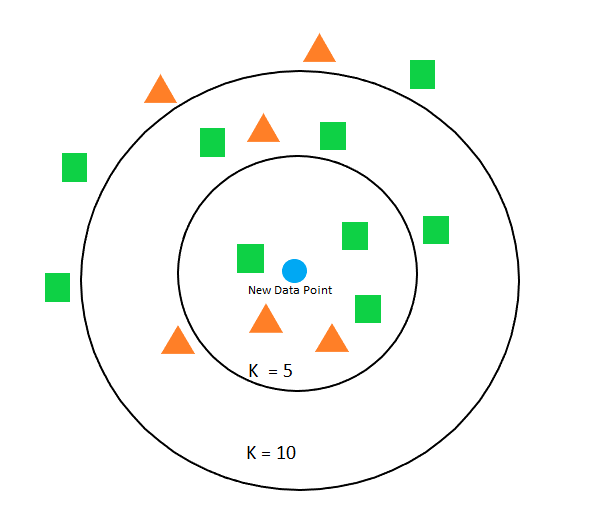
\includegraphics[width=10cm]{kNN.png}
    \caption{Przykład klasyfikacji przy pomocy algorytmu KNN}
    \label{fig:knn}
\end{figure}

\newpage %% dlaczego nowa sekcja nie rozpoczyna sie od nowej kartki? nani?

\section{Stworzenie rankingu cech}
Przygotowanie pełnego rankingu cech jest na tym etapie projektu nie możliwe. Zgodnie z metodą 2-krotnej walidacji krzyżowej, która polega na dzieleniu zbioru danych na zbiór danych do uczenia algorytmu, oraz testowania, nie jest możliwe wyznaczenie jednego optymalnego rankingu cech. Możliwe jest wykonanie obliczeń na wszystkich obiektach każdej klasy, jednak zaburza to założenie nieznajomości zbioru wykorzystywanego do testowania na etapie uczenia modelu.

W naszym projekcie zdecydowaliśmy się na użycie algorytmu filtrowania cech $\chi^2$-distribution. Algorytm chi-squared został wybrany z powodu lepszego radzenia sobie ze zmiennymi nie-ciągłymi spośród wszystkich dostępnych algorytmów w bibliotece \texttt{scikit-learn}.

Ranking cech stworzony na podstawie wszystkich obiektów znajduje się w Tab. \ref{tab:feature-ranking-table}.

\begin{center}
	\begin{longtable}{ |c|c|c| } 
		\hline
			Numer cechy & Nazwa cechy & Wartość $\chi^2$ \\
		\hline
			35 & Systolic blood pressure & 1980.234530 \\
			6 & Number of hours since onset & 978.577747 \\
			2 & Pain location & 340.518254 \\
			53 & New ST segment depression & 223.468210 \\
			49 & New Q wave & 200.255889 \\
			55 & New T wave inversion & 193.397661 \\
			51 & New ST segment elevation & 188.224104 \\
			54 & Any ST segment depression & 176.999688 \\
			57 & New intraventricular conduction defect & 159.891546 \\
			56 & Any T wave inversion & 151.671957 \\
			38 & Respiration rate & 120.295290 \\
			43 & Diastolic murmur & 117.164923 \\
			58 & Any intraventricular conduction defect & 117.095337 \\
			21 & Prior angina prectoris & 116.642864 \\
			3 & Chest pain radiation & 114.724420 \\
			37 & Heart rate & 109.556062 \\
			50 & Any Q wave & 108.815692 \\
			45 & S3 gallop & 105.087366 \\
			17 & Prior pain related to heart & 101.630463 \\
			18 & Prior pain due to MI & 89.168603 \\
			46 & S4 gallop & 87.110979 \\
			19 & Prior pain due to angina prectoris & 85.870499 \\
			23 & Congestive heart failure & 85.265596 \\
			42 & Systolic murmur & 84.497398 \\
			25 & Hiatal hernia & 83.614284 \\
			12 & Dizziness/syncope & 83.285357 \\
			10 & Palpitations & 82.348879 \\
			31 & Beta blockers & 79.733144 \\
			36 & Diastolic blood pressure & 78.562607 \\
			30 & Nitrates & 76.574549 \\
			52 & Any ST segment elevation & 75.294437 \\
			34 & Antacids/H2 blockers & 73.567453 \\
			7 & Duration of the last episode & 63.415290 \\
			32 & Digitalis & 60.113284 \\
			40 & Cyanosis & 58.805874 \\
		\hline
		\caption{35 najlepszych cech wg rankingu wyznaczonego dla wszystkich obiektów}
		\label{tab:feature-ranking-table}
	\end{longtable}
\end{center}


\bibliographystyle{plain}
\end{document}
